\documentclass[border=10pt]{standalone}

\usepackage{tikz}
\usepackage{tikzsymbols}
\usetikzlibrary{calc,patterns,shapes.geometric}

\def\centerarc[#1](#2)(#3:#4:#5){\draw[#1] ($(#2)+({#5*cos(#3)},{#5*sin(#3)})$) arc (#3:#4:#5);}

\begin{document}
	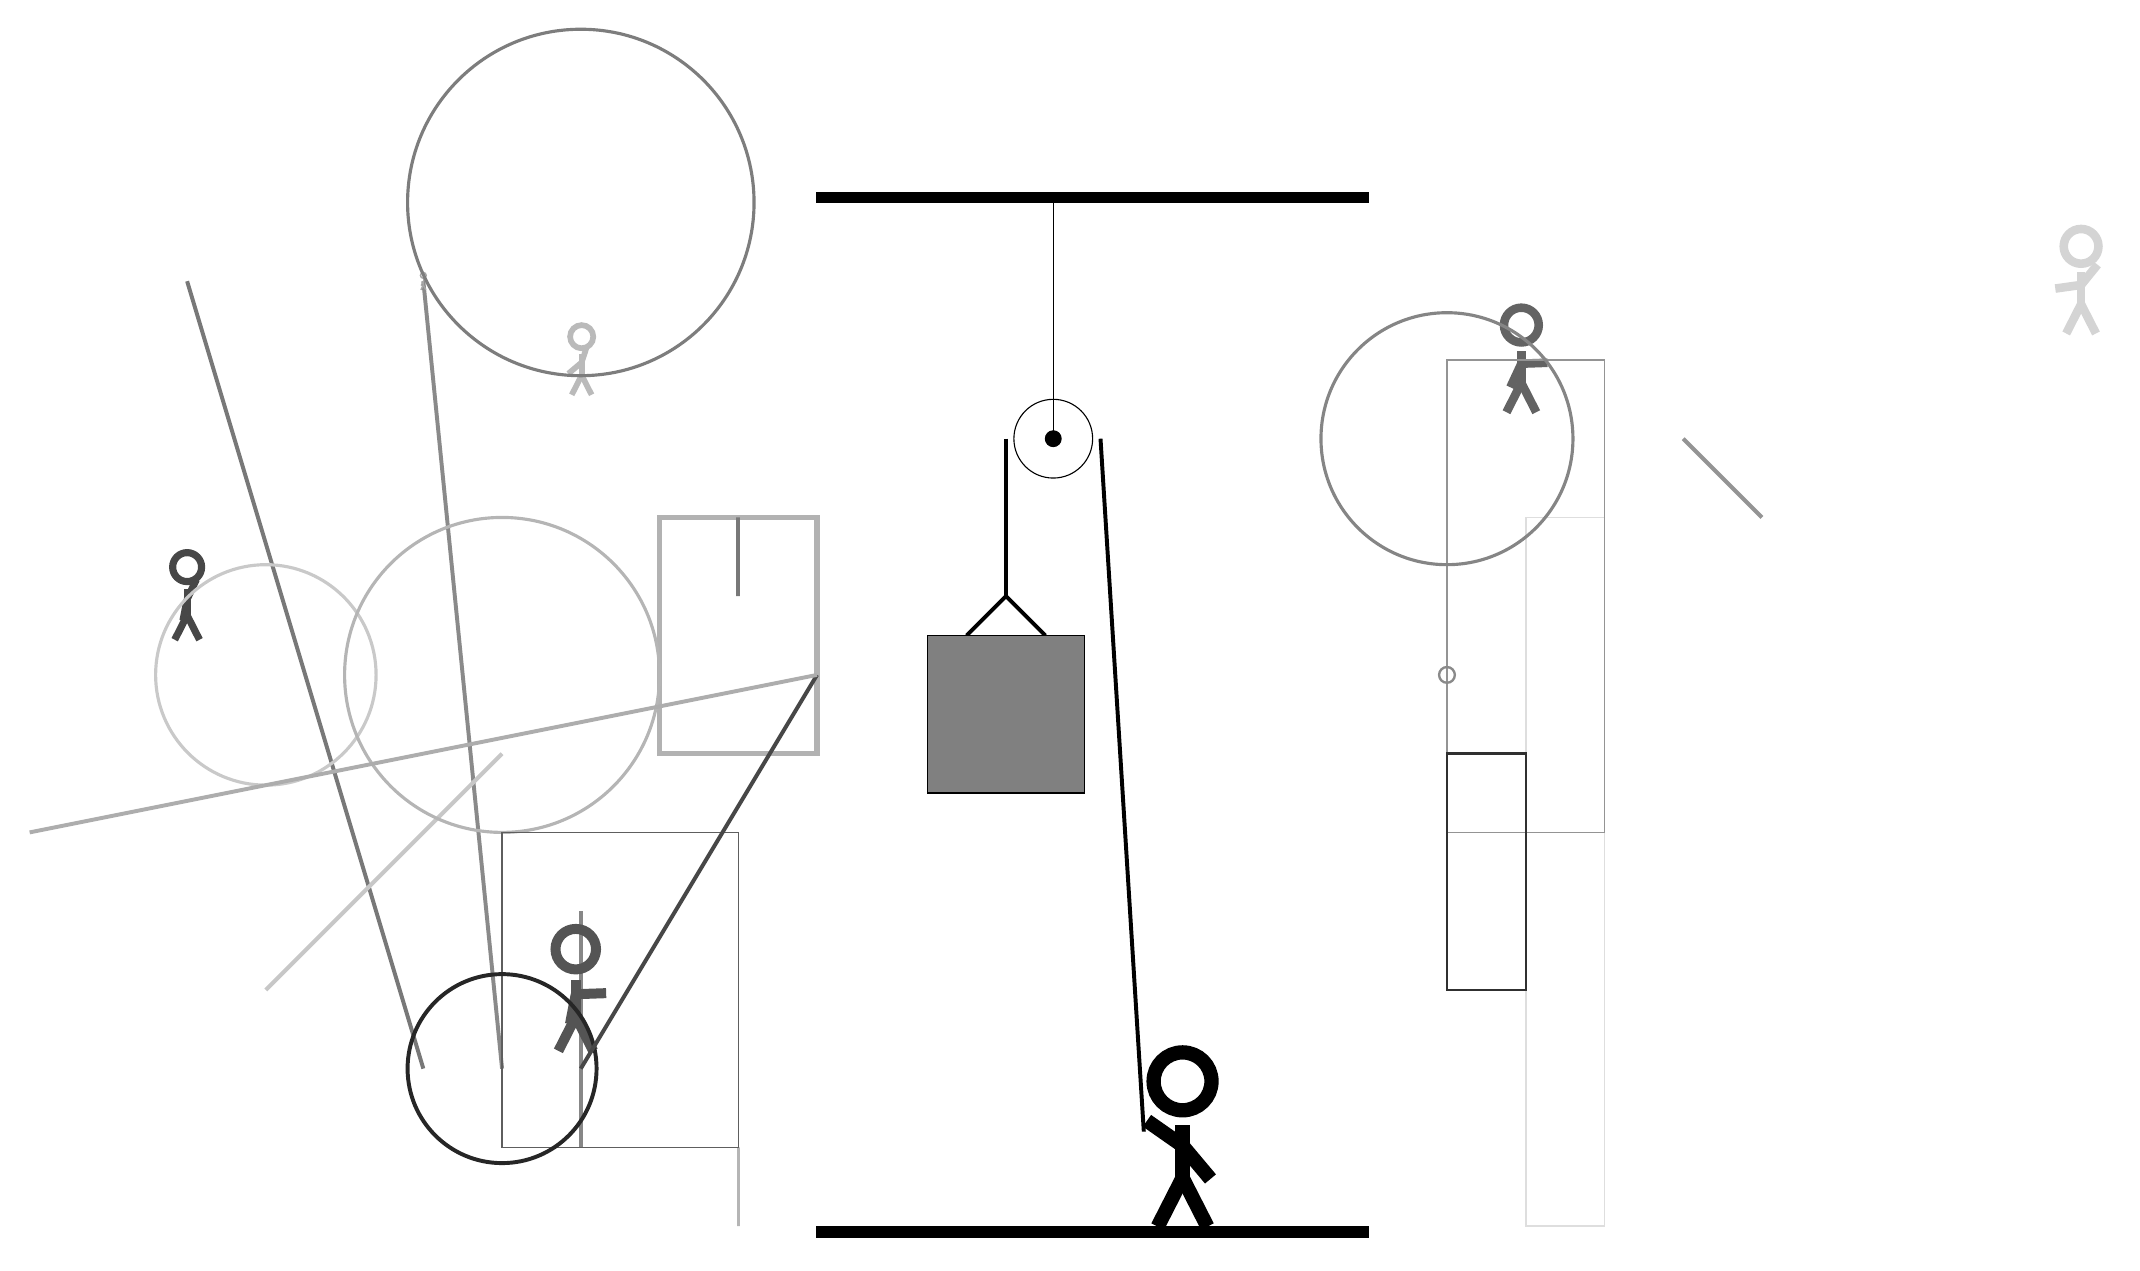
\begin{tikzpicture}
		%%%%% START %%%%%
		
		\draw[fill=black] (-2, 10) rectangle (5, 10.125);
		
		\draw (1, 7) circle (0.5);
		\draw[fill=black] (1, 7) circle (0.1);
		\draw (1, 10) -- (1, 7);
		
		\draw[line width=0.5mm] (-0.1, 4.5) -- (0.4, 5.0) -- (0.9, 4.5);
		\draw[fill=black!50] (-0.6, 4.5) rectangle (1.4, 2.5);
		
		\draw[line width=0.5mm] (0.4, 7) -- (0.4, 5.0);
		\centerarc[line width=0.5mm](1, 7)(0:180:0.6);
		\draw[line width=0.5mm](1.6, 7) -- (2.15, -1.8);
		
		\draw[line width=0.5mm, color=black!46](-7, 9) -- (-6, -1);
		
		\node[line width=0.7mm, color=black!35] at (-7, 9) {\Strichmaxerl[1][59][76]};
		\node[line width=0.6mm, color=black!17] at (14, 9) {\Strichmaxerl[6][8][51]};
		\node[line width=0.6mm, color=black!72] at (-10, 5) {\Strichmaxerl[5][79][65]};
		\draw[line width=0.5mm, color=black!47](-5, 1) -- (-5, -2);
		
		\draw[line width=0.2mm, color=black!13] (7, 6) rectangle (8, -3);
		\draw[line width=0.5mm, color=black!53](-7, -1) -- (-10, 9);
		\draw [line width=0.4mm, color=black!21](-9, 4) circle (1.4);
		\draw[line width=0.7mm, color=black!30] (-2, 6) rectangle (-4, 3);
		\node[line width=0.2mm, color=black!61] at (7, 8) {\Strichmaxerl[6][65][2]};
		\draw[line width=0.2mm, color=black!42] (6, 8) rectangle (8, 2);
		
		\draw[line width=0.5mm, color=black!22](-6, 3) -- (-9, 0);
		\draw[line width=0.5mm, color=black!42](10, 6) -- (9, 7);
		
		\draw [line width=0.4mm, color=black!29](-6, 4) circle (2.0);
		\draw[line width=0.3mm, color=black!81] (6, 3) rectangle (7, 0);
		\draw[line width=0.4mm, color=black!29] (-3, -2) rectangle (-3, -3);
		\draw [line width=0.4mm, color=black!48](6, 7) circle (1.6);
		
		\node[line width=0.4mm, color=black!67] at (-5, 0) {\Strichmaxerl[7][79][2]};
		\node[line width=0.4mm, color=black!27] at (-5, 8) {\Strichmaxerl[4][40][72]};
		\draw[line width=0.2mm, color=black!63] (-3, -2) rectangle (-6, 2);
		\draw [line width=0.4mm, color=black!51](-5, 10) circle (2.2);
		\draw [line width=0.5mm, color=black!85](-6, -1) circle (1.2);
		\draw[line width=0.5mm, color=black!72](-2, 4) -- (-5, -1);
		\draw [line width=0.3mm, color=black!46](6, 4) circle (0.1);
		\draw[line width=0.5mm, color=black!53] (-3, 5) rectangle (-3, 6);
		\draw[line width=0.5mm, color=black!32](-2, 4) -- (-12, 2);
		
		
		\node at (2.6, -1.9) {\Strichmaxerl[10][-35][-50]};
		
		\draw[fill=black] (-2, -3) rectangle (5, -3.15);
		
		%%%%% END %%%%%
	\end{tikzpicture}
\end{document}